\section{Introduction}
\label{section:intro}

Distributed architectures have witnessed a significant increase of interest
during the last decade, as the number of interconnected computers increased, the
available digital information kept proliferating, at an exponetial rate each
year, and problems to be addressed by IT became more and more demanding. Why is
there a correlation, and it is not just a coincidence? Distributed computation
suggests a simple paradigm\footnote{Of course, as always, this is the case only
after someone thought about it first!}. Get a set of autonomous computing
entities and put them to cooperate with each other in order to fullfil a well
defined task. In the World of the Internet and the World Wide Web this also
offers a thrilling promise. To harness the immence power scattered across the
Internet and get amply rewarded by exploiting the data, storage and
computational resources out there.

In order to achieve that, computers collaborate by exchanging messages via an
application-level network where they can address each other in the specific
context of the task at hand. This communication structure is refered to as an
\emph{overlay network} which is an abstract, logical inter-connection formed on
top of another network\footnote{The Internet itself is an overalay on top of the
telephone network.}. It consists of a set of nodes, the computing elements, that
are being connected by virtual (logical) point-to-point links, perhaps
corresponding to multiple physical links. Figure~\ref{figure:overlay}
illustrates a simple four-node overlay contructed upon a wide area network.

\begin{figure}
\centering
  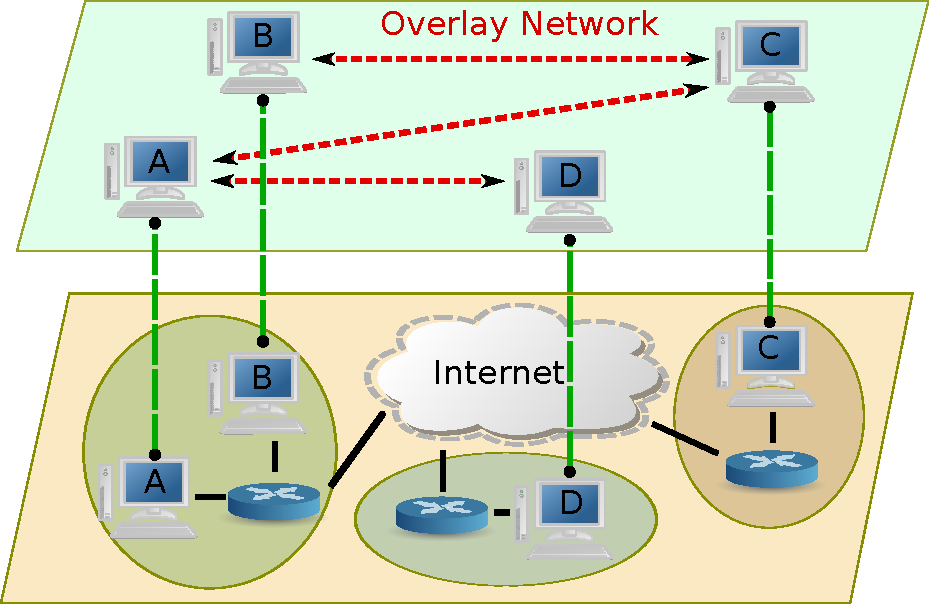
\includegraphics[scale=0.5]{img/p2p.pdf}
\caption{An example overlay network.}
\label{figure:overlay}
\end{figure}

The abstraction of the overlay network has been proposed as a way to implement
efficient, fully distributed, application-layer services. For example, backing
the routing of messages to destinations that are not known in advance or
building one-to-many addressing schemes
% TODO find citation for Narada & Adobe's Real Time Media Flow Protocol (RTMFP)
\cite{} that would provide higher quality-of-service (QoS) guarantees. \emph{IP
multicast}, as well as other proposals such as \emph{IntServ} and
\emph{DiffServ} \cite{cisco_diffserv_2005}, have not seen wide acceptance
(yet?), largely due to the fact they require support from the physical
infrastructure. On the other hand, an overlay network can be deployed on
end-systems running the overlay protocol software, without cooperation from the
ISPs.
%Academic research includes
%\cite{chu_esm_2000,jannotti_overcast_2000,kwon_tag_2002} among others.

%%%%%%%%%%%%%%%%%%%%%%%%%%%%%%%%%%%%%%%%%%%%%%%%%%%%%%%%%%%%%%%%%%%%%%%%%%%%%%%%
%%%%%%%%%%%%%%%%%%%%%%%%%%%%%%%%%%%%%%%%%%%%%%%%%%%%%%%%%%%%%%%%%%%%%%%%%%%%%%%%
\subsection{Peer-to-Peer (P2P) Architectures in a Nutshell}
%%%%%%%%%%%%%%%%%%%%%%%%%%%%%%%%%%%%%%%%%%%%%%%%%%%%%%%%%%%%%%%%%%%%%%%%%%%%%%%%
%%%%%%%%%%%%%%%%%%%%%%%%%%%%%%%%%%%%%%%%%%%%%%%%%%%%%%%%%%%%%%%%%%%%%%%%%%%%%%%%
Overlay networks on top of the best-effort IP layer, formed a widely ranged
family of protocols collectively known as \emph{peer-to-peer} or \emph{P2P} for
short. P2P systems consist of a number of networked computers called
\emph{peers}, where each, such, \emph{peer} could act both as a resource
provider and a resource consumer. This changed the traditional
\emph{client-server} model dominating the Internet and lead to the introduction
of the \emph{servent} concept \cite{gnutella}, a \emph{portmanteau} that blends
the notions of server and client to denote the twofold role of the P2P network
participants. Such serverless systems, proved to be able to achieve outstanding
aggregate resource capacities as more and more participants join the system
without requiring additional expenditure for infrastructure\footnote{
  Unfortunatelly, there has been observed mitigation of this self-scaling
  property by the undesirable behaviour of participating users, usually answered
  in popular file-sharing systems; from \emph{free-riding}

\cite{saroiu_measurefileshare_2002,adar_gnutellafreeriders_2000,hughes_gnutellafreeride_2005}
to the distribution of illegal content and/or other \emph{socio-technical}
issues \cite{hughes_socp2p_2008}.
}.
P2p network systems gained extra attention whithin the distributed systems
super-set, circa 2000, due to the fact that they succesfully supported popular
applications that offered file sharing among vast numbers of participating
users. But their development didn't stay still. On the contrary, during the last
decade, research on P2P systems was constant and fruitfull generating a wide
range of popular protocols, networks and applications. As P2P systems evolved
three main architectures have been emerged, namely
\begin{inparaenum}[\itshape i\upshape)]
  \item \emph{centralized},
  \item \emph{decentralized unstructured}, and
  \item \emph{decentralized structured}.
\end{inparaenum}

\emph{Centralized} architectures (see Figure~\ref{figure:p2p-archs:centralised})
were the first to recognize that requests for resourses (e.g. CPU cycles
\cite{seti} or popular content
% TODO find citation for Napster
\cite{}) need not be sent to a dedicated server but instead could be handled by
the many hosts that already posses them. This schema, though, is not fully
distributed since it dictates a centralised searching facility, a characteristic
that can be proven its ``Achilles' heel'' in terms of being a scalability
bottleneck, a central point of failure and vulnerable to malicious acts (e.g.
\emph{Denial-of-Service (DoS) attacks}).

The centralized approach has been eventually replaced by architectures that
distributed both search and download capabilities (see
Figures~\ref{figure:p2p-archs:unstructured-full} and
\ref{figure:p2p-archs:unstructured-hierarchical}). In these \emph{decentralized}
architectures, file placement is random, which means there is no correlation
with the network topology whatsoever \cite{yang_improvep2psearch_2002}. For this
reason they are also refered to as \emph{unstructured}. The most important
properties of such systems are that they support inherent heterogeneity of
peers, are highly resilient to peer failures, and incur low maintenance overhead
at handling the dynamics of peer participation \cite{stutzbach_churn_2006}. In
the literature, they are also known as \emph{broadcast-based} systems, because
they use \emph{message flooding} among peers or super-peers to propagate
queries.
%\footnote{The life of each query message is constrained by an integer, refered
%to as \emph{time-to-live (TTL)}. When a querry is received by a (super-) peer,
%this value is decreased by one unit. Then, the receiver, back-propagates its
%results and if the TTL has not reached zero the node forwards the query message
%to all its neighbours except from the one it received it from.}


Recently, \emph{decentralized structured} schemes have been proposed (see
Figure~\ref{figure:p2p-archs:structured}) in order to provide a self-organising
infrastructure for large-scale P2P applications
\cite{ratnasamy_can_2001,stoica_chord_2001,antony_pastry_2001,zhao_tapestry_2001,maymounkov_kademlia_2002,rgrk_bamboo_2004}.
They implement a \emph{Distributed Hash Table (DHT)} that maps objects to nodes
through a deterministic mechanism. Even though unstructured networks became
highly popular among file sharing applications, they do have a certain
limitation in locating rare objects. The DHT approach of structured networks on
the other hand, provides a guaranteed bound on the number of overlay routing
hops that have to be taken in order for an object to be located, even in the
case where only a single copy exists in the system.  This means
$O \left ( log n \right )$ hops, compared to unstructured networks that require
$O \left ( n \right )$ to reliably locate a specific object\footnote{
  Unfortunatelly this efficiency does not come without cost. Structured overlays
  realise what is called object identifier location as opposed to content-based
  retrieval of unstructured ones. This means that the later can support more
  versatile object location mechanisms like keyword and partial matching
  searches.}.

% TODO: Change these pictures to match look-n-feel
\begin{figure}[ht]
\centering
\subfigure[Centralised (SETI@Home or Napster).] {
  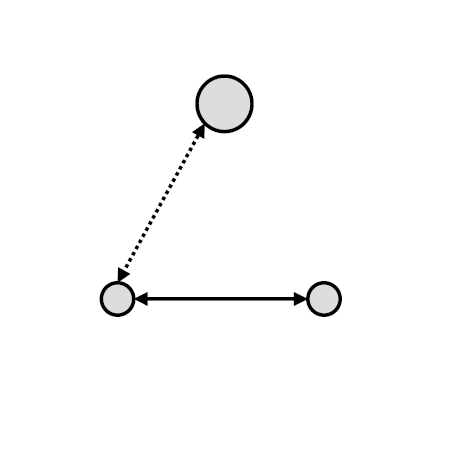
\includegraphics[scale=0.3]{img/centralised.png}
  \label{figure:p2p-archs:centralised}
}\qquad\qquad
\subfigure[Fully unstructured (Gnutella v.0.4).] {
  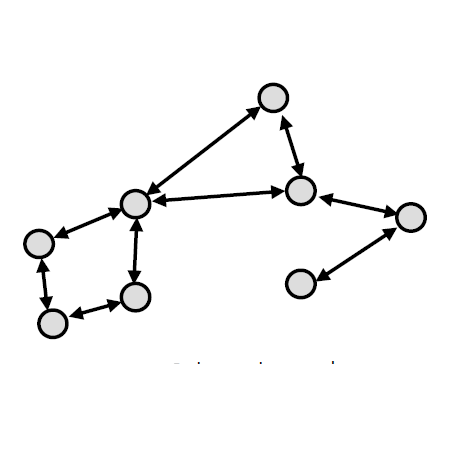
\includegraphics[scale=0.3]{img/unstructured-full.png}
  \label{figure:p2p-archs:unstructured-full}
}\qquad\qquad
\subfigure[Hierarchical unstructured (Gnutella v.0.6 or FastTrack).] {
  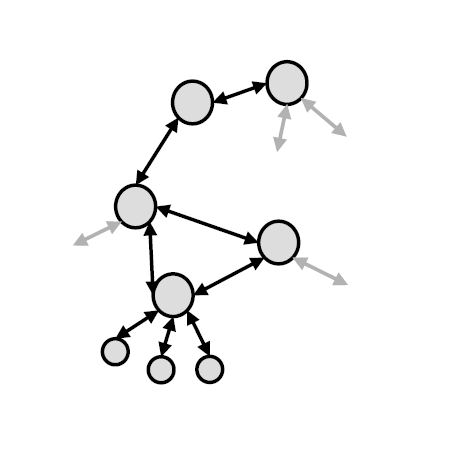
\includegraphics[scale=0.3]{img/unstructured-hierarchical.png}
  \label{figure:p2p-archs:unstructured-hierarchical}
}\qquad\qquad
\subfigure[Structured (Chord and Kademlia).] {
  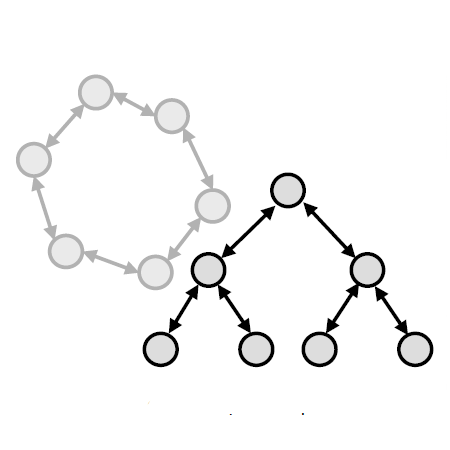
\includegraphics[scale=0.3]{img/structured.png}
  \label{figure:p2p-archs:structured}
}
\caption{The various peer-to-peer architectures.}
\label{figure:p2p-archs}
\end{figure}

%%%%%%%%%%%%%%%%%%%%%%%%%%%%%%%%%%%%%%%%%%%%%%%%%%%%%%%%%%%%%%%%%%%%%%%%%%%%%%%%
%
% TODO: SOME DISCUSSION ON P2P ARCHITECTURES
%
%\cite{matei_mapgnutella_2002, lv_randomwalks_2002, merugu_str2unstr_2003}
%showed that the ad-hoc network topology of unstructured overlay networks that
%preserve \emph{Power Law} and \emph{Small World} characteristics\footnote{Power
%Law describes the node degree while the Small World describes characteristics
%of path length and clustering coefficient. The clustering coefficient for a
%node $\upsilon$ in a graph $G = \left( V, E \right)$ is defined as the ratio of
%the existing connections between $\upsilon$'s neighbouring nodes to $\gamma
%\times \left( \gamma - 1 \right)$, where $\gamma$ is the number of neighbouring
%nodes of $\upsilon$. High cluster coefficient means that neighbouring nodes of
%any node $\upsilon$ likely connect one another.} \cite{faloutsos_powerlaw_1999,
%saroiu_measurefileshare_2002} offer a more promising approach. Particularly:
%\begin{itemize}
%  \item Peer-to-peer clients are extremely \emph{transient}. Unstructured
%systems can have high maintenance traffic in delivering messages, updating the
%mapping, discovering failures and replicating lost data or pointers, making
%them insufficient on highly volatile networks.
%  \item \emph{Keyword searches} versus \emph{exact-match queries}. In DHTs
%there is a tight control between the data placement and the topology of the
%network. For this reason it is hard to efficiently support partially matched
%queries while Gnutella and other similar systems effortlessly support keyword
%searches and other complex queries since the mechanism is realized locally, on
%a node-by-node basis.
%  \item Popular content is located at multiple peers and thus it is more likely
%for a flooding-based search to return results. DHTs, on the other hand, fit
%better in the systems which require ability to reliably locate content, even in
%the extreme case that only a single-copy exists in the network.
%\end{itemize}

%
% TODO: SOME DISCUSSION ON THE ADVANTAGES OF UNSTRUCTURED NETWORKS FROM
%       \cite{z-yk_ddno_2005}
%
%Unstructured P2P networks o?er a number of
%important advantages: (i) An unstructured network
%imposes very small demands on individual nodes,
%and more speci?cally it allows nodes to join or leave
%the network without signi?cantly a?ecting the sys-
%tem performance. (ii) Unstructured networks are
%appropriate for content-based retrieval (e.g., key-
%word searches) as opposed to object identi?er loca-
%tion of structured overlays. (iii) Finally unstructured
%networks can easily accommodate nodes of vary-
%ing power. Consequently, they scale to very large
%sizes and they o?er more robust performance in
%the presence of node failures and connection
%unreliability.
%

%
% TODO: SOME DISCUSSION ON STRUCTURED OVERLAYS PROBABLY FROM
%       \cite{wu_laptop_2007}
% However, the design of a decentralized but structured P2P network has to
% overcome two critical issues. The first issue is the long routing latency.
% Several proximity schemes  have been proposed to avert long routing latency in
% current structured P2P networks, but they require a high-complexity procedure
% to periodically maintain the routing table (e.g. Pastry system) or they need
% pre-chosen landmarks to construct the overlay. However, the P2P system is by
% its very nature unstable since nodes join and leave frequently. For instance,
% the study of Gnutella shows around approximately 1200 membership changes per
% minute in a 100 000 nodes P2P system. Another proximity scheme needs some
% pre-chosen landmarks or a complete BGP routing table support. As a result,
% they both increase the difficulty of the P2P system deployment. The second
% issue is system maintenance overhead. The existing structured P2P networks
% allow nodes to keep some nearby nodes in their routing tables in order to
% achieve efficient routing.
%


%%%%%%%%%%%%%%%%%%%%%%%%%%%%%%%%%%%%%%%%%%%%%%%%%%%%%%%%%%%%%%%%%%%%%%%%%%%%%%%%

%%%%%%%%%%%%%%%%%%%%%%%%%%%%%%%%%%%%%%%%%%%%%%%%%%%%%%%%%%%%%%%%%%%%%%%%%%%%%%%%
%%%%%%%%%%%%%%%%%%%%%%%%%%%%%%%%%%%%%%%%%%%%%%%%%%%%%%%%%%%%%%%%%%%%%%%%%%%%%%%%
\subsection{Applications and Implications}
%%%%%%%%%%%%%%%%%%%%%%%%%%%%%%%%%%%%%%%%%%%%%%%%%%%%%%%%%%%%%%%%%%%%%%%%%%%%%%%%
%%%%%%%%%%%%%%%%%%%%%%%%%%%%%%%%%%%%%%%%%%%%%%%%%%%%%%%%%%%%%%%%%%%%%%%%%%%%%%%%

The most successful incarnation of the centrilised approach is without a doubt
the popular file-sharing application \emph{Napster}\footnote{Pioneering, though,
was the famous \emph{SETI@Home Project} \cite{seti}, which pools spare
processing power of participants to search the universe for the existence of
extra terrestrial intelligence!}
% TODO find citation for Napster again
\cite{}.
Napster maintained a \emph{central index server} based on file lists provided by
participating peers. The central index server was queried by the users and it
returned pointers to the actual content. Thus, by centralizing search while
distributing downloads, Napster achieved a highly functional design that was
widely acknowledged, at the time, as ``the fastest growing Internet application
ever'' that toped some 26 million users and 80 million songs
\cite{jmm_naptopusage_2001}.

Napster was ultimatelly brought down after Recording Industry Association of
America (RIAA) filed a lawsuit for copyright infringement of the intellectual
property of artists whose music was distributed by the network\footnote{
  The sueing spree was initiated by heavy metal giants \emph{Metallica} that
  feared Napster was undermining record sales. Opposed opinions instantly
  emerged with best example the british alternative rock band \emph{Radiohead}
  whose album \emph{Kid A} had also been leaked to Napster three months before
  reaching music store shelves \cite{rm_radioheadkida_2000}. Despite music
  critics labeling the album ``experimental'' and ``challenging'' (it had no
  official singles nor music videos for any of its songs), in October 2000 Kid A
  captured the number one spot on the Billboard 200 sales chart in its debut
  week. Unlike Metallica, Madonna and Dr.Dre that led litigation with Napster,
  Radiohead had never hit the top20 in the US before.
}
\cite{wiki_amnaptrial_2001}. This triggered a shift towards decentralised
networks like the classic \emph{Gnutella} and, its ``rival'' at the time,
\emph{FastTrack}. Gnutella, in its first realisation (v.0.4 \cite{gnutellav04}),
was a fully decentralised approach. Unfortunatelly, network resourses tended to
be overwhelmed by message flooding and if queries were constrained to live for
some (small) number of hops, this ultimatelly resulted to a shrinked search
scope, leading to a death spiral that prevented the network from scaling. The
solution came with a slightly more structured network by introducing the notions
of \emph{ultra-peers} and \emph{leaf-nodes} (v.0.6 \cite{gnutella}). With
\emph{Limewire}, the most widely used software that implemented the protocol,
the network was highly successful and was reported to have reached connecting
more that 3 million users concurrently by the end of 2006
\cite{rsr_gnutellaevol_2006}. Fasttrack and its implementing software KaZaA
\cite{kazaa}, on the other hand, went with the hierarchical approach
(\emph{super-nodes} in their context) from the very begining, dynamically
assigning indexing functions to special peers in order to increase search
performace and scaling potential. FastTrack network had an average of 3 million
concurrently connected nodes in 2003 \cite{lkxr_kazaameasure_2005}. It is
estimated that the total number of users was greater than that of Napster at its
peak. With Limewire discontinued/shutdown in 2010 and its successor,
\emph{Frostwire}, moving to the Bittorent protocol in 2011, seem to very well
signal the end of the once-mighty Gnutella network. KaZaA continues as a
propriatery music store solution. In the meanwhile, Fastrack design team had
already introduced a VoIP and text messaging application based on the design
principles of KaZaA's hierarchical P2P nature, that was meant to change how
people communicate around the world. This app was no other than Skype
\cite{skype}. Despite its wide usage, little is known for the technical aspects
of its overlay network, mainly due to its proprietary nature. Studies, though,
confirm that it shares strong structural similarities to its file-sharing
predecessor (ordinary hosts and super-nodes in Skype's terminology) but they
significantly differentiate in terms of traffic behaviour
\cite{g_voipskypesec_2005,gdj_skypestudy_2006}. Skype was introduced in 2003
and from then on it witnessed frenzy-rythmed increase to its popularity, with
more that 650 milion registered users in 2011 \cite{skypetotalusers} and
reported to have broken the barrier of 35 million skypers concurrently online on
the the 5th of March 2012 \cite{skypesymusers}. On October 2011 Microsoft Corp.
and Skype Global S.à.r.l. anounnced the completion of Microsoft's acquisition of
Skype for \$$8.5$ billion \cite{skypemicrosoft}.

File sharing was the most popular application area for structured architectures
as well. Overnet
% TODO find citation for Overnet
\cite{},
for example, was created for sharing large files (e.g., movies and CD images).
It implemented the Kademlia tree-like partitioning algorithm. Other
implementations of Kademlia are the Kad Network (eMule/aMule  clients),
BitTorrent for trackerless torrernts (official BitTorrent client, $\mu$Torrent,
BitComet, Transmission and BitSpirit all share compatibility with the Mainline
DHT which realises the Kademlia protocol) and the Gnutella DHT (first
implemented by LimeWire as the Mojito DHT). Lately, RetroShare \cite{retroshare}
is the new trend for file-sharing which incorporates an implementation of the
Kademlia DHT to create a Friend-to-Friend (F2F) network with some attributes of
a darknet as well. But the potential of structured architectures was not
exhausted only to the above. Structured P2P networks became popular in
distributed systems because they could scale smoothly and have fast and reliable
object location mechanisms. Thus, research and development was very active and
productive resulting in a variety of diverse applications such like distributed
search engines \cite{yaci}, distributed data storage systems
\cite{kbc_oceanstore_2000,bdet_fsdfs_2000,dkkms_cfs_2001,dr_pastutility_2001,abc_farsite_2002,mmfc_ivy_2002,arla,agebh_dks_2003}, Web caches, archives,
and publishing systems \cite{ird_squirrel_2002,bags_youserv_2002,wrc_publius_2000,wm_tangler_2001},
messaging applications \cite{threedegrees}, event notification infrastructures
\cite{rkcd_scribe_2001,cdkr_scribe_2002,agebh_dks_2003}, naming services
\cite{cmm_chorddns_2002}, censor-resistent stores \cite{cswh_freenet_2001} and
lately even cloud-based platforms \cite{mgpj_cloudsnap_2011}.

%%%%%%%% NEW TRENDS %%%%%%%%
%File sharing Limewire Kazzaa The file-sharing landscape is slowly adjusting in
%response to the continued push for more anti-piracy tools, the final Pirate Bay
%verdict, and the raids and arrests in the Megaupload case, SOPA, ACTA. This
%leads to users trying to find new solutions for anonymous, uncensored,
%decentralised file sharing solutions like Freenet, Tribler and RetroShare where
%connections are made only between trusted peers — sometimes called "friends"
%and the respective formed network F2F.

% TODO: READ Dalesa published at eAsia 2009, http://www.e-asia.org/2009/ET_Presentations/Wathsala.pdf

The huge numbers of users, for the various applications we presented above,
reveals the tremendous popularity P2P architectures have enjoyed. This, though,
does not come without any toll. Measurements on some popular systems, such as
FastTrack, Gnutella, DirectConnect and BitTorrent have shown that the P2P
traffic contributes the largest portion of the overall Internet traffic
\cite{seroiu_analysiscds_2002,sen_analyzep2ptraffic_2004,krp_ispfear_2005}.
Even with later studies, this observation still holds on. Using deep packet
inspection techniques deployed at selected customer sites \emph{Ipoque} and
\emph{CacheLogic} were able to track down application usage \cite{cachelogic,ipoque2007,ipoque2009}.
CacheLogic reports that more than 60\% of the traffic is identified as P2P, with
Ipoque verifying this observation reporting similar results for 2007, while
observing some small decline for 2008/2009 (but still remaining dominant
compared to other applications). Apart from its participation in overall usage
terms, P2P is already a huge contibutor to the overall data exchanged across the
Internet\footnote{
  Mainly because file-sharing P2P is used to exchange big files of HD video or
  high sampled audio content compared to simple Web content distributed via, for
  example, HTTP.
}.
\cite{multinteligence} claims that P2P traffic in 2007 was around 1.6 petabytes
per month and the potential is to be quintubled by the end of 2012 reaching
almost 8 petabytes per month.

%
% TODO: SOME DISCUSSION from \cite{zhao_ctag_2006}
%
%%Observations made in various studies (e.g. \cite{matei_mapgnutella_2002})
% concerning the distribution of nodes among \emph{Internet Service Providers
%(ISPs)} and \emph{Autonomous Systems (ASs)} have shown that only $2$ to $5$
%percent of Gnutella connections link peers within a single AS while more than
%$40$ percent of all Gnutella peers are located within the top 10 ASs.
%Similarly, measurements in \cite{zeinalipour-yazti_gnudc_2002} used a $244,000$
%IPs test-bed and results have shown that $45$ percent of the nodes belonged to
%only $10$ large ISPs and $58$ percent belong to only $20$. Such results mean
%that most overlay generated traffic crosses AS borders increasing topology
%mismatch cost.

%%%%%%%%%%%%%%%%%%%%%%%%%%%%%%%%%%%%%%%%%%%%%%%%%%%%%%%%%%%%%%%%%%%%%%%%%%%%%%%%
%%%%%%%%%%%%%%%%%%%%%%%%%%%%%%%%%%%%%%%%%%%%%%%%%%%%%%%%%%%%%%%%%%%%%%%%%%%%%%%%
\subsection{The Topology Mismatch Problem}
%%%%%%%%%%%%%%%%%%%%%%%%%%%%%%%%%%%%%%%%%%%%%%%%%%%%%%%%%%%%%%%%%%%%%%%%%%%%%%%%
%%%%%%%%%%%%%%%%%%%%%%%%%%%%%%%%%%%%%%%%%%%%%%%%%%%%%%%%%%%%%%%%%%%%%%%%%%%%%%%%

One of the major issues that defines the efficiency of an overlay network is the
mapping of the overlay structure to the underlying infrastructure. Remember, in
Figure~\ref{figure:overlay} Nodes $A$ and $B$ are on the same local network,
while $C$ and $D$ are in different networks. The top layer represents the
overlay interconnection formed by these nodes at a higher level. Link
connections there, can change as needed by the running environment, without any
particular constraint by the underlying physical topology. Let's have a closer
look with the help of a simple example. Assume nodes $A$, $B$, $C$ and $D$ are
connected through the physical network shown in Figure~\ref{figure:phys}, where
the network costs are given in milliseconds, and peer $A$ sends a message to
peer $D$.

\begin{figure}
\centering
  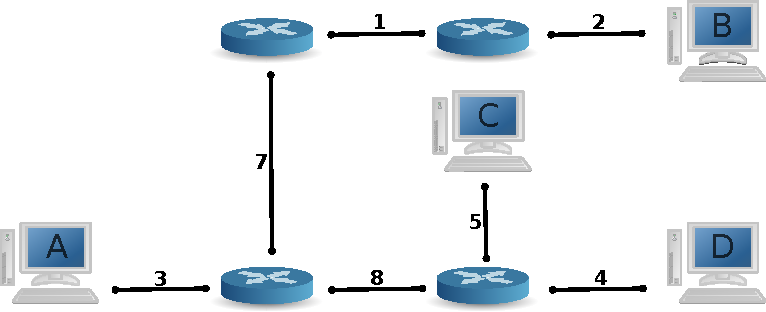
\includegraphics[scale=0.8]{img/phys.pdf}
\caption{Interconnection of nodes in the physical level.}
\label{figure:phys}
\end{figure}

If these peers participate in an overlay network according to one of the setups
of Figure~\ref{figure:overlay-confs} then users will expierience different
performances. In the overlay depicted in Figure~\ref{figure:overlay-1}, the
message will traverse the following sequence of links in the physical layer
(marked with their costs): $3 \rightarrow 7 \rightarrow 1 \rightarrow 2
\rightarrow 2 \rightarrow 1 \rightarrow 7 \rightarrow 8 \rightarrow 5
\rightarrow 5 \rightarrow 4$. In the alternative overlay of Figure
~\ref{figure:overlay-2}, the path will be: $3 \rightarrow 8 \rightarrow 4$. The
total cost of the first sequnce is $45 ms$, while the second yields a mere $15
ms$. Therefore, we can conclude that the second overlay is more congruent with
the underlying physical network than the first one and, thus, is more efficient.

\begin{figure}[ht]
\centering
\subfigure[Nodes B and C have direct overlay connection.] {
  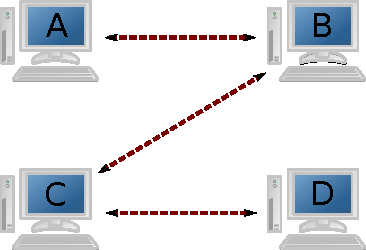
\includegraphics[scale=0.8]{img/overlay-1.pdf}
  \label{figure:overlay-1}
}\qquad\qquad
\subfigure[Nodes A and D have direct overlay connection.] {
  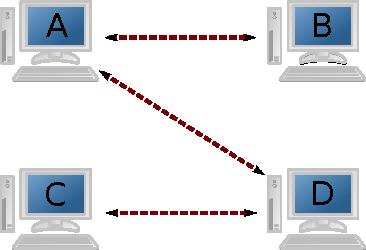
\includegraphics[scale=0.8]{img/overlay-2.pdf}
  \label{figure:overlay-2}
}
\caption{Two different overlay connection configuration.}
\label{figure:overlay-confs}
\end{figure}

Ideally, overlay networks are expected to achieve an optimal mapping among the
overlay paths and the underlying physical links, and avoid inefficient states.
The problem of constructing an optimal overlay is referred to as the
\emph{topology mismatch problem}, and formally defined as follows:
\begin{definition}
Let $V = \{v_1, ..., v_n\}$ be a set of points denoting the network nodes,
$\{v_i, v_j\} \in E$ be the set of unicast distances between nodes $v_i$ and
$v_j$, $G=(V,E)$ be a complete distance graph over $V$. The topology mismatch
problem is to construct a minimal spanning tree,  where node degree is
restricted to a constant ($k\geq 2$) by the bandwidth of each node $v_i$.
\end{definition}

Early incarnations of the overlay protocols, however, did not make use of the
optimal mapping with the physical network topology. Gnutella protocol for
example was considered far from scalable \cite{ritter_gnucantscale_2001}. Since
every peer can chοse its logical neighbours without knowledge of the underlying
network had as a result a mismatch between physical and application-level
topologies. Additionally, queries may be flooded to multiple paths merging in
one peer while in such case one of the paths would have been enough.
Nevertheless, peers may forward the same message to each other before they
receive the query messages from each other. \cite{matei_mapgnutella_2002} showed
that, even given that 95\% of any two nodes are less than 7 hops away from each
other, a flooding-based algorithm, like the one used by Gnutella, can generate
330TB/month in a 50.000 node network! Therefore, P2P traffic can have a serious
effect on the overall well-being of the Internet as a whole.

Similar problems are observed in decentralized structured schemes also.
Typically, node IDs are assigned \emph{randomly}, resulting in excellent load
balancing, scalability and robustness. Unfortunately, this randomness has a
negative impact on the \emph{routing locality} of the network. This means that
even though the target node can be reached with logarithmic overlay hops, the
distance traveled in the physical underlying network, during the overlay routing
process, can be far from optimal.  The ratio of the physical distance, a query
travels through the overlay to an object, and the minimal distance to that
object (i.e. through IP) is known in the literature as \emph{stretch} or
\emph{Relative Delay Penalty (RDP)} \cite{chu_esm_2000}.

%%%%%%%%%%%%%%%%%%%%%%%%%%%%%%%%%%%%%%%%%%%%%%%%%%%%%%%%%%%%%%%%%%%%%%%%%%%%%%%%
%%%%%%%%%%%%%%%%%%%%%%%%%%%%%%%%%%%%%%%%%%%%%%%%%%%%%%%%%%%%%%%%%%%%%%%%%%%%%%%%
\subsection{Motivation and our Goal for this Survey}
%%%%%%%%%%%%%%%%%%%%%%%%%%%%%%%%%%%%%%%%%%%%%%%%%%%%%%%%%%%%%%%%%%%%%%%%%%%%%%%%
%%%%%%%%%%%%%%%%%%%%%%%%%%%%%%%%%%%%%%%%%%%%%%%%%%%%%%%%%%%%%%%%%%%%%%%%%%%%%%%%
A topology unaware overlay network is able to control the sequence of peers a
message traverses before reaching its destination, but it is completely unaware
of how the actual packets are switched at the underlying infrastructure along
the overlay path. For example, a single logical point-to-point link on the
overlay, most of the time, corresponds to multiple physical links in the
underlying layer. Additionally, a link in the underlying network often serves
the mapping of several overlay paths causing increase of the traffic on the
physical link, which is also called the link's \emph{stress}\cite{chu_esm_2002}.
Furthermore, the network's \emph{churn}, that is the stochastic behaviour of
peers randomly joining and leaving the P2P network, all cause the overlay to
physical mapping to create such unnecessary, redundant maintenance traffic that
impacts the efficiency of the network in terms of average response time.

The topology mismatch problem is exacerbated by the high amounts of traffic
generated by the highly popular P2P applications. This creats the killer
combination for the network infrastructure, ultimately effecting all Internet
users. Solving it, on the other hand, is no easy task. Topology mismatch is
known to be an NP-Hard problem \cite{NPBOOK,chawathe_scattercast_2000}.
Moreover, the Internet itself is an interesting environment where end-to-end
latencies demonstrate what is called \emph{triangle inequality violations
(TIVs)}, which further complicate the problem. These delay space TIV is a
consequence of the Internet's structure and routing policies and thus will
remain a property of the Internet for the foreseeable future
\cite{zheng_irprtt_2005}. TIVs affect network coordinate
\cite{cox_vivaldi_2004,wong_meridian_2005} and positioning \cite{ng_gnp_2001}
and makes the construction of location/delay aware overlays difficult. An
extensive array of heuristic approaches have been proposed in an effort to find
an algorithm that performs reasonably and consistently well. The purpose of this
survey is to gather the extensive knowledge that has been produced recently in
this research field and organise the available information ultimately helping
the reader sift through the myriad of these efforts, understand the different
approaches and identify though a taxonomy the advantages and disadvantages of
each of them.

%
% TODO: SOME DISCUSSION FROM \cite{xu_globstate_2003) CONTRADICTS TO THE
%TRIANGLE INEQUALITY ARGUMENT ABOVE
%
%[snip]
%Studies [14] have shown that triangle inequality may not hold in Internet
%topology. In fact, study from Pastry has shown that the proximity approximation
% is much worse when using the Mercator topology that is based on the real
% measurements of the Internet [3].
%

%%%%%%%%%%%%%%%%%%%%%%%%%%%%%%%%%%%%%%%%%%%%%%%%%%%%%%%%%%%%%%%%%%%%%%%%%%%%%%%%
%%%%%%%%%%%%%%%%%%%%%%%%%%%%%%%%%%%%%%%%%%%%%%%%%%%%%%%%%%%%%%%%%%%%%%%%%%%%%%%%
\subsection{Survey Outline}
%%%%%%%%%%%%%%%%%%%%%%%%%%%%%%%%%%%%%%%%%%%%%%%%%%%%%%%%%%%%%%%%%%%%%%%%%%%%%%%%
%%%%%%%%%%%%%%%%%%%%%%%%%%%%%%%%%%%%%%%%%%%%%%%%%%%%%%%%%%%%%%%%%%%%%%%%%%%%%%%%

% TODO: Review this after the content and article structure is fixed.
In the introduction we had the oportunity to recognise the importance of overly
networks in contemporary application architectures. Also we quickly reviewed the
basic trends in both overlay construction\footnote{
  The main focus of this paper is the topology mismatch problem, therefore the
  available approaches in overlay networks are briefly summarized, and
  interested readers are pointed to the available surveys on overlay networks
  \cite{TheotokisS04,LuaCPSL05}.
}
and application development. Last but not least, we identified and formaly
defined the phenomenon of the topology mismatch problem and its impact on the
utilization of network resources. The rest of the survey\ldots

Sections~\ref{sec:unstructured} and \ref{sec:structured} discuss the recent
academic work that has been conducted in the field.

Ultimately, it reviews the most important resources found in the literature that
attempt to tackle the problem as it proposes a taxonomic scheme, using a set of
supertype-subtype relationships based on unique characteristics they have and/or
specific goals they target. What follows does not claim to be a thorough
citation of all known protocols that are available out there, but instead, a
careful selection of those that left a distinctive fingerprint contribution in
the efforts of the research community to alleviate the topology mismatch
problem.